\section{Left-Right}
\label{sec:LR}

	This section will describe the fitting modes that can handle determining the left-right sides of the hits within the fitting. The first and shorter section describes the ``mainFit'' fit mode and the second and longer section describes the ``fullSeqFit'' fit mode. Some of this information is repeated from the GeaneFittingUtils.cc section describing these fit modes. It is important to remember that while some left-right information for the track may be determined upstream, most of it cannot until a fit of some sort is completed. For us that is the wire fit, which does not require any left-right information in order to work. The wire fit serves as the starting point for determing the left-right sides of the hits since the overall fit will approximately get the left-right sides correct, though not always. Even a single hit side being incorrect can throw the fit off, which is usually readily apparent with resulting high $\chi^{2}$s or low p-values. Sometimes this incorrect side (or sides) can be determined by looking at the individual plane $\chi^{2}$s and finding the outliers, though this is not always the case. Due to the smearing of the real dcas from the straw resolution, sometimes it can be very difficult to determine the left-right sides in all hits. There is planned to be a refinement stage in the future, which will be tasked with adjusting the track that is to be fitted, both dealing with left-right sides and removing or adding hits to the fit. Until such a time however, we are unable to fit all tracks correctly with 100\% fidelity due to this left-right ambiguity problem.

	\subsection{mainFit}

	  First a wire fit is completed with a couple of iterations. Then a fit is performed where each iteration takes as its hit sides wherever the previous fit ended up. Something like 2/3rds of the tracks converge nicely with this method, but not all. (In the current iteration of the code there is also an intermediate second wire fit, where the known sides from the doublet geometry and track angle are set, which helps salvage a couple of tracks.) If the left-right sides are only taken from the wire fit a single time, instead of being updated each iteration, then less tracks converge.

	\subsection{fullSeqFit}

      This fitting mode takes the longest time to fit a track, because it checks every single left-right combination for all hits in order to find the best track. It starts by first doing a wire fit in order to get approximate track objects (transport matrices, error matrices, predicted parameters) used for making approximate guesses at how good different left-right combinations are. It takes those approximate track objects and a particular combination of left-right choices for the individual hits and constructs a $\chi^{2}$ for that combination. The set of best $\chi^{2}$s corresponding to the best left-right combinations are then saved. One can also lock certain hits to left, right, or center depending on how the user is fitting (locking left-right from known geometry, small dcas, etc), and the track fitting will loop over the remaining unknown sides, checking each combination. In order to increase the speed of this code greatly, instead of checking all $2^{N}$ combinations directly, the $2^{Nu}$ and $2^{Nv}$ combinations are checked separately (leaving the other measured parameter sides as being set to the wires). See Figure \ref{fig:SeqCheckSteps} for a diagramatic view of exactly how this approximate fitter works for the sequence checking, and read the \hyperref[sec:GeaneLRUtils]{GeaneLRUtils.cc} section for detail on the methods that are used within the fullSeqFit.

			\begin{figure}[]
				\caption{This figure shows the steps used to determine an approximate set of the best U and V left-right sequences. Note that these steps are followed separately but identically for U and V. The equations here are identical to some of those given in the \hyperref[sec:Formalism]{Formalism} section. The sequenceChecking method of the \hyperref[sec:GeaneFitter]{GeaneFitter} class is where this is completed in the code. Step 1 is performing a wire fit, done once for all $2^{N}$ U or V combinations. The resulting generated transport, error, and covariance matrices along with the predicted parameters from the wire fit are saved for the following steps. Step 2 involves using those aforementioned matrix objects, but now with the measured positions in the calculation replaced with whatever particular left-right sequence is being checked. An approximate fix to the track is then calculated, which can be used in step 3 to determine a new set of approximate predicted parameters. These approximate predicted parameters are then combined with the measured left-right sequence that's being checked in step 4, along with a hybrid error matrix (where if U sequences are being checked, then the V planes have wire errors, and vice versa) to calculate an approximate $\chi^{2}$ for that particular sequence. All U and V sequences are checked and the best 10, with the lowest $\chi^{2}$s, of each are saved. The arrows show where matrix objects are used from one step to another. This method while still slow for many combinations, especially high N tracks, is pretty fast because it's simple matrix multiplication over and over again, without actually Geane fitting eaching $2^{N}$ combination. (And no inversions.) Note that while not as effective, it is possible to jump from step 1 to step 4, where the predicted parameters remain as those predicted from the wire fit, and calculate an approximate $\chi^{2}$ for the left-right sequence. This has the benefit of being faster by skipping steps 2 and 3 but fails for more events, and so isn't as useful.}
				\hspace{10 mm}
				\centering
				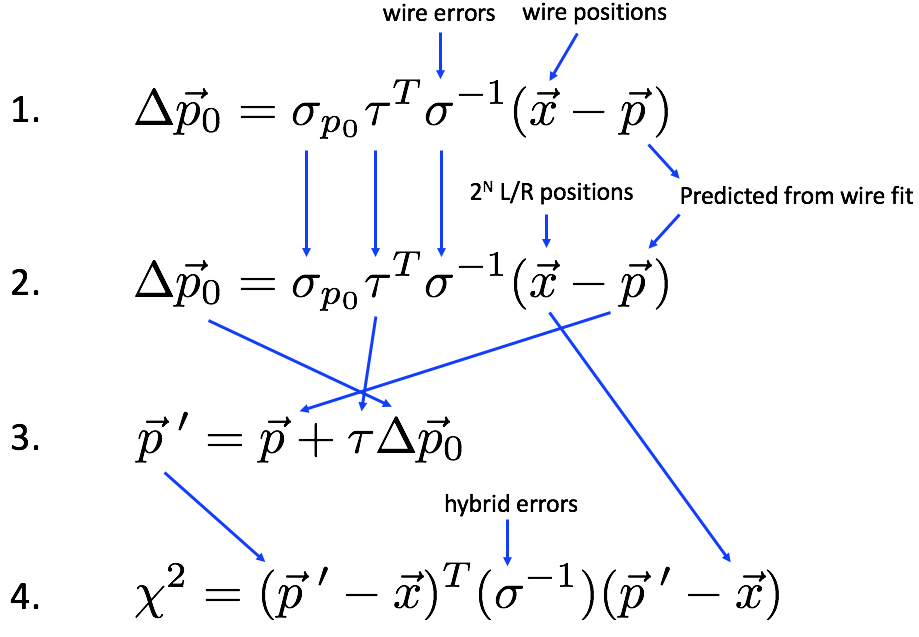
\includegraphics[width=0.8\textwidth]{SeqCheckSteps}
				\label{fig:SeqCheckSteps}
			\end{figure}

 	  Once the set of best U and V sequences have been determined with the approximate fitter, they are combined together and fitted with the full Geane error propagation fitting. For a small sample of fitted tracks, Figure \ref{fig:PositionOfBest} shows where in the set of best 10 saved $\chi^{2}$s for the different sequences the actual truth sequence is. (For a larger sample of tracks, this plot would fill out more with less empty bins.) It can be seen that the approximate fitter actually guesses the correct U and V sequences a large percentage of the time. When combining the U and V sequences together and full fitting, it is beneficial to scan over some smaller set instead of the full 10 by 10 grid. (Sometimes the approximate fitter can fail to save the correct left-right combination at all if the dca smearing is too large.) The red line in the figure separates out a set of 15 tracks to full fit, which results in high fidelity of fitted tracks. If one wishes an even smaller set of tracks can be full fitted, where more tracks will result in poor fits, but the speed of the tracking improves significantly. See \href{https://gm2-docdb.fnal.gov/cgi-bin/private/ShowDocument?docid=6800}{DocDB 6800} for a quick study of track fitting speed vs the level of results, where one should pay attention to the number of tracks within the 0 bin of the p-value plots, representing poorly fit tracks coming from incorrectly chosen left-right sequences. 

 	  It is also possible to cut short the sequences that are being full fitted. When there is a couple of very similar sequences, possibly with small dcas, the track fitting results in similar $\chi^{2}$s. Usually soon after there is a large jump in the full fitted track $\chi^{2}$ as some left-right choices have been changed, revealing that that particular sequence and the ones after are incorrect. For example the $\chi^{2}$s might go as 10.2, 11.4, 10.3, 38.9..., and it is at this large jump that one can make a reasonable assumption that the best sequence has been found. This of course does not work perfectly all of the time but it is a good way of eking some more speed out of the tracking. The user can configure the fitting (from base fcl parameters to options such as described here) to optimize vs fit results or speed however desired. This should be combined and studied with the future refinement stage. One might wish to do faster fits to start and refine the poorly fitted tracks before doing more thorough sequence checking and the like.

			\begin{figure}[]
				\caption{The fullSeqFit mode saves the smallest 10 $\chi^{2}$s from the approximate fitter for the ``best'' U and V sequences. For the set of 10 best U sequences, the X bins in this plot represent the location of the true U sequences, and similarly for V. For example, if the 0 bin is filled then the U sequence with the smallest $\chi^{2}$ is the true sequence, if the 1 bin is filled then the U sequence with the second smallest $\chi^{2}$ is the true sequence, etc. It can be seen that the approximate fitter does a very good job of actually guessing the true U and V sequences with the bottom 3 bins holding most of the events. Some sequences do end up in the higher bins where the approximate fitter has not done so good of a job at determing the true left-right sequences, including some events which end up in the overflow bins where the approximate fitter has simply failed. The angled red line describes a region of combined sequences to perform the full fitting over in order to try and find the combined true left-right sequence. Note that even then the true sequence may not have the smallest $\chi^{2}$ in the final fitting due to the smearing of dcas. Note also that hit digits with very small dcas will have very similar $\chi^{2}$s and fill neighboring bins, though this fact is ignored when locking small dcas to the wire centers.}
				\centering
				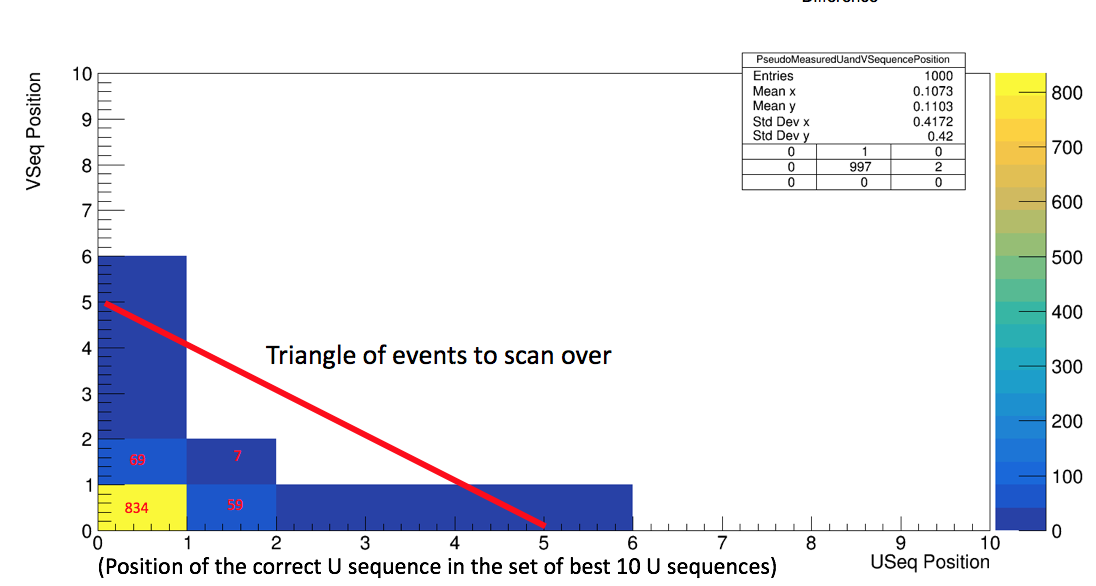
\includegraphics[width=1.0\textwidth]{PositionOfBest}
				\label{fig:PositionOfBest}
			\end{figure}
